\slide{Plan}
{
% NOTE: each line starting with '% NOTE:' will be exported as a 'script.log', along with the section and file names.
% NOTE: this is a nice way of making a notes for you presentation.
% NOTE: ex. explain the plan in detail - forcus on point 4.
\tableofcontents
}

% note that this way you can easily comment-out compleated sections, when working on the document.
% this signifficantly speeds up work. oh - and use 'make fast' target for compiltion - it will run latex just once.
% it may result in incorrect indexes and numbers missmatch, but for a preview is just fine.
\section{Text}


\slide{Text in multiple comulns}
{
% NOTE: talk alot here, as there is no point in doing anything usefull
% NOTE: do not sleep
% NOTE: remember to eat something
\begin{multicols}{2}
Lorem ipsum dolor sit amet, consectetur adipisicing elit, sed do eiusmod tempor incididunt ut labore et dolore magna aliqua. Ut enim ad minim veniam, quis nostrud exercitation ullamco laboris nisi ut aliquip ex ea commodo consequat. Duis aute irure dolor in reprehenderit in voluptate velit esse cillum dolore eu fugiat nulla pariatur. Excepteur sint occaecat cupidatat non proident, sunt in culpa qui officia deserunt mollit anim id est laborum.
\end{multicols}
}


\slide{Points}
{
\begin{itemize}
\item Item 1
\pause

\item Item 2
\begin{enumerate}
\item Enum 1
\item Enum 2
\end{enumerate}
\end{itemize}
}


\slide{Columns}
{
\begin{columns}

\begin{column}{0.45\textwidth}
\begin{itemize}
\item Alice
\item Has
\item A
\item Cat
\end{itemize}
\end{column}

\begin{column}{0.45\textwidth}
\begin{itemize}
\item Cat
\item Has
\item AIDS
\end{itemize}
\end{column}

\end{columns}
}


\slide{Message boxes}
{
\begin{block}{Famous quote}
Lorem ipsum dolor sit amet, consectetur adipisicing elit, sed do eiusmod tempor incididunt ut labore et dolore magna aliqua.
\end{block}
}


\slide{Font sizes}
{
\tiny{tiny} \\
\scriptsize{scriptsize} \\
\footnotesize{footnotesize} \\
\small{small} \\
\normalsize{normalsize} \\
\large{large} \\
\Large{Large} \\
\LARGE{LARGE} \\
\huge{huge} \\
\Huge{Huge}
}


\slide{Any questions so far?}
{
\begin{center}
\vspace{-10em}
\fontsize{160}{200}\selectfont ?
\end{center}
}


\slide{Verbatim blocks}
{
\begin{itemize}
\item \emph{verbatim} does not work normally
\item \emph{fragile} does not work when inside \emph{newcommand}
\item \emph{semiverbatim} is prefferred
\item it may require some escaping though\ldots
\end{itemize}
\begin{semiverbatim}
some weird +!@\% text

it's fine \
\end{semiverbatim}
}


\slide{UTF-8 characters}
{
\begin{itemize}
\item \url{http://www.johndcook.com/unicode\_latex.html}
\item maps unicode -> \LaTeX "dings":
\begin{itemize}
\item check mark: \ding{52} (ding 52)
\item x mark: \ding{56} (ding 56)
\end{itemize}
\item not my idea -- sorry folks...
\end{itemize}

\begin{columns}

\begin{column}{0.45\textwidth}
\begin{center}
\color{red}
\fontsize{60}{70}\selectfont
\ding{56}
\end{center}
\end{column}

\begin{column}{0.45\textwidth}
\begin{center}
\color{green}
\fontsize{60}{70}\selectfont
\ding{52}
\end{center}
\end{column}

\end{columns}
}

\section{Subsections}


\slide{section 1 start}
{
\begin{multicols}{2}
HELLO \\
Lorem ipsum dolor sit amet, consectetur adipisicing elit, sed do eiusmod tempor incididunt ut labore et dolore magna aliqua. Ut enim ad minim veniam, quis nostrud exercitation ullamco laboris nisi ut aliquip ex ea commodo consequat. Duis aute irure dolor in reprehenderit in voluptate velit esse cillum dolore eu fugiat nulla pariatur. Excepteur sint occaecat cupidatat non proident, sunt in culpa qui officia deserunt mollit anim id est laborum.
\end{multicols}
}


\subSlide{section 1 cont}
{
\begin{multicols}{2}
STILL WORKING \\
Lorem ipsum dolor sit amet, consectetur adipisicing elit, sed do eiusmod tempor incididunt ut labore et dolore magna aliqua. Ut enim ad minim veniam, quis nostrud exercitation ullamco laboris nisi ut aliquip ex ea commodo consequat. Duis aute irure dolor in reprehenderit in voluptate velit esse cillum dolore eu fugiat nulla pariatur. Excepteur sint occaecat cupidatat non proident, sunt in culpa qui officia deserunt mollit anim id est laborum.
\end{multicols}
}


\subSlide{section 1 end}
{
\begin{multicols}{2}
DONE HERE! \\
Lorem ipsum dolor sit amet, consectetur adipisicing elit, sed do eiusmod tempor incididunt ut labore et dolore magna aliqua. Ut enim ad minim veniam, quis nostrud exercitation ullamco laboris nisi ut aliquip ex ea commodo consequat. Duis aute irure dolor in reprehenderit in voluptate velit esse cillum dolore eu fugiat nulla pariatur. Excepteur sint occaecat cupidatat non proident, sunt in culpa qui officia deserunt mollit anim id est laborum.
\end{multicols}
}


\slide{section 2 start}
{
\begin{multicols}{2}
HELLO \\
Lorem ipsum dolor sit amet, consectetur adipisicing elit, sed do eiusmod tempor incididunt ut labore et dolore magna aliqua. Ut enim ad minim veniam, quis nostrud exercitation ullamco laboris nisi ut aliquip ex ea commodo consequat. Duis aute irure dolor in reprehenderit in voluptate velit esse cillum dolore eu fugiat nulla pariatur. Excepteur sint occaecat cupidatat non proident, sunt in culpa qui officia deserunt mollit anim id est laborum.
\end{multicols}
}


\subSlide{section 2 cont}
{
\begin{multicols}{2}
STILL WORKING \\
Lorem ipsum dolor sit amet, consectetur adipisicing elit, sed do eiusmod tempor incididunt ut labore et dolore magna aliqua. Ut enim ad minim veniam, quis nostrud exercitation ullamco laboris nisi ut aliquip ex ea commodo consequat. Duis aute irure dolor in reprehenderit in voluptate velit esse cillum dolore eu fugiat nulla pariatur. Excepteur sint occaecat cupidatat non proident, sunt in culpa qui officia deserunt mollit anim id est laborum.
\end{multicols}
}


\subSlide{section 2 end}
{
\begin{multicols}{2}
DONE HERE! \\
Lorem ipsum dolor sit amet, consectetur adipisicing elit, sed do eiusmod tempor incididunt ut labore et dolore magna aliqua. Ut enim ad minim veniam, quis nostrud exercitation ullamco laboris nisi ut aliquip ex ea commodo consequat. Duis aute irure dolor in reprehenderit in voluptate velit esse cillum dolore eu fugiat nulla pariatur. Excepteur sint occaecat cupidatat non proident, sunt in culpa qui officia deserunt mollit anim id est laborum.
\end{multicols}
}

\section{Listings}


\slide{Test module}
{
\begin{itemize}
\item Modules end with "-m"
\item They are self-containing
\end{itemize}
\lstinputlisting{cpp/test-m.hpp}
}


\slide{Test function}
{
\begin{itemize}
\item Functions ends with "-f"
\item Content of file is wrapped into a function call
\end{itemize}
\lstinputlisting{cpp/other-f.hpp}
}


\slide{Multicolumn listing}
{
\tiny{}
\begin{multicols}{2}
\lstinputlisting{cpp/long_source-m.hpp}
\end{multicols}
}


\slide{Highlighted listing}
{
\only<1>{ \lstinputlisting{cpp/some_function-f.hpp} }
\only<2>{ \highlightedListing{1}{1}{cpp/some_function-f.hpp} }
\only<3>{ \highlightedListing{2}{2}{cpp/some_function-f.hpp} }
\only<4>{ \highlightedListing{3}{3}{cpp/some_function-f.hpp} }
\only<5>{ \highlightedListing{5}{8}{cpp/some_function-f.hpp} }
\only<6>{ \highlightedListing{3}{3}{cpp/some_function-f.hpp} }
\only<7>{ \highlightedListing{5}{8}{cpp/some_function-f.hpp} }
\only<8>{ \highlightedListing{11}{11}{cpp/some_function-f.hpp} }
}

\section{Graphics}


\slide{Full-slide image}
{
\insImgCenter{0.25}{pic/transistor}
\sourceRefUrl{https://upload.wikimedia.org/wikipedia/commons/e/e2/Transistor-die-KSY34.jpg} % image source (creative common license)
}


\slide{Image with source-reference link shifted}
{
\insImg{-0.30}{0.12}{0.31}{pic/transistor}
\insImg{0.50}{0.12}{0.25}{pic/transistor}
\vspace{15em}
\sourceRefUrlShifted{50em}{https://upload.wikimedia.org/wikipedia/commons/e/e2/Transistor-die-KSY34.jpg} % image source
}


\slide{Box around image part}
{
\begin{center}
\begin{tikzpicture}
\node[anchor=south west, inner sep=0] at (0,0) { 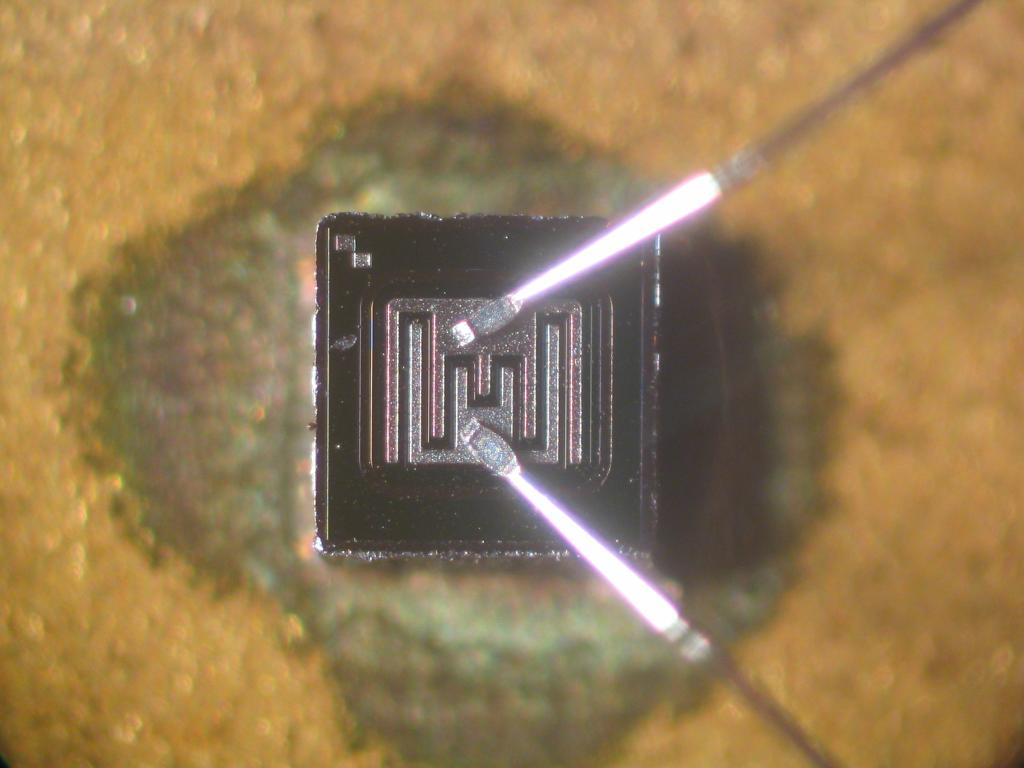
\includegraphics[scale=0.25]{pic/transistor} };
\draw<1>[green,thick,       rounded corners] (2.7, 1.6) rectangle (\textheight-3.2cm, 5);
\draw<2>[red,  ultra thick, rounded corners] (3.9, 2.5) rectangle (4.8, 3.2);
% NOTE: rectangle ++(0.8, 0.4); is an offset, instead of an abs poisiton
\end{tikzpicture}
\end{center}
\sourceRefUrl{https://upload.wikimedia.org/wikipedia/commons/e/e2/Transistor-die-KSY34.jpg} % image source (creative common license)
}


\slide{Images on the same page}
{
\begin{center}
\includegraphics<1>[scale=0.125]{pic/transistor}
\pause
\includegraphics<2>[scale=0.25]{pic/transistor}
\end{center}
\sourceRefUrl{https://upload.wikimedia.org/wikipedia/commons/e/e2/Transistor-die-KSY34.jpg} % image source (creative common license)
}


\slide{Image decorations}
{
\begin{itemize}
\item Lorem ipsum dolor sit amet,
\item consectetur adipisicing elit,
\item sed do eiusmod tempor incididunt
\item ut labore et dolore magna aliqua.
\item Ut enim ad minim veniam, quis
\item nostrud exercitation ullamco laboris
\item nisi ut aliquip ex ea commodo consequat.
\item Duis aute irure dolor in reprehenderit
\item in voluptate velit esse cillum dolore
\item eu fugiat nulla pariatur.
\end{itemize}
\insImg{0.8}{0.2}{0.05}{pic/transistor}
\pause

\insImgFr{2-}{0.8}{0.55}{0.08}{pic/transistor}
}


\slide{Images interleaved with text}
{
Lorem ipsum dolor sit amet, consectetur adipisicing elit, sed do eiusmod tempor incididunt ut labore et dolore magna aliqua.

\begin{center}
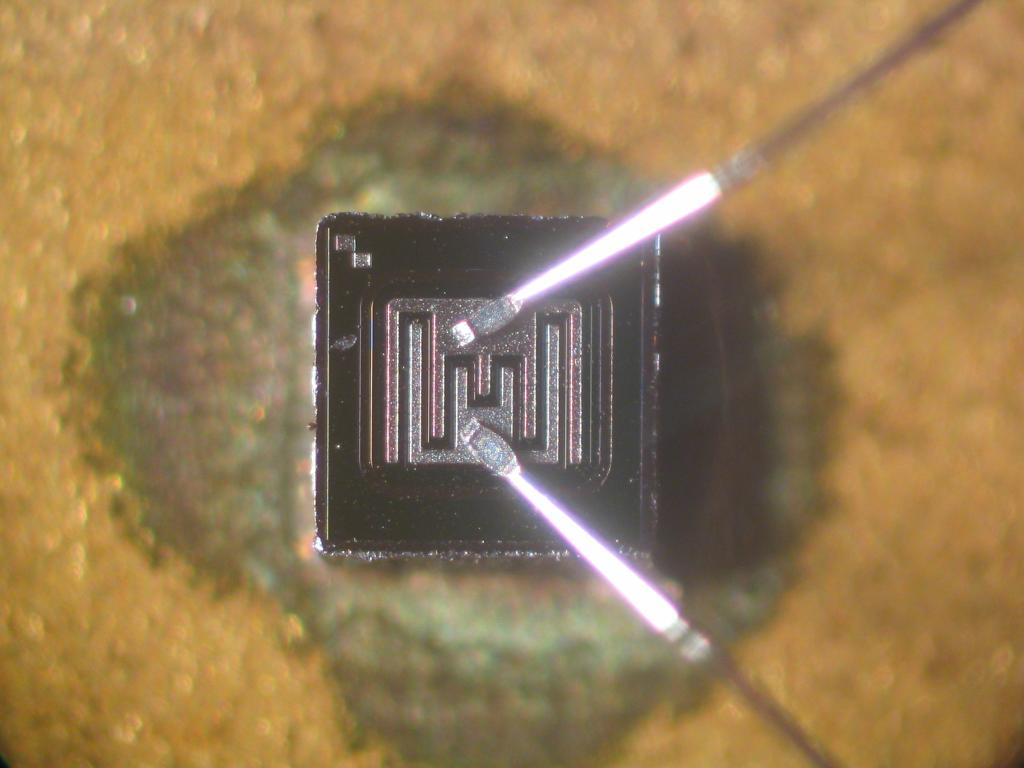
\includegraphics[scale=0.1]{pic/transistor}
\end{center}

Ut enim ad minim veniam, quis nostrud exercitation ullamco laboris nisi ut aliquip ex ea commodo consequat.
}


\slide{PNGs out of SVGs}
{
\begin{center}

\includegraphics[scale=0.5]{svg/biohazard}
\end{center}
}


\slide{} % unnamed!
{
\begin{center}
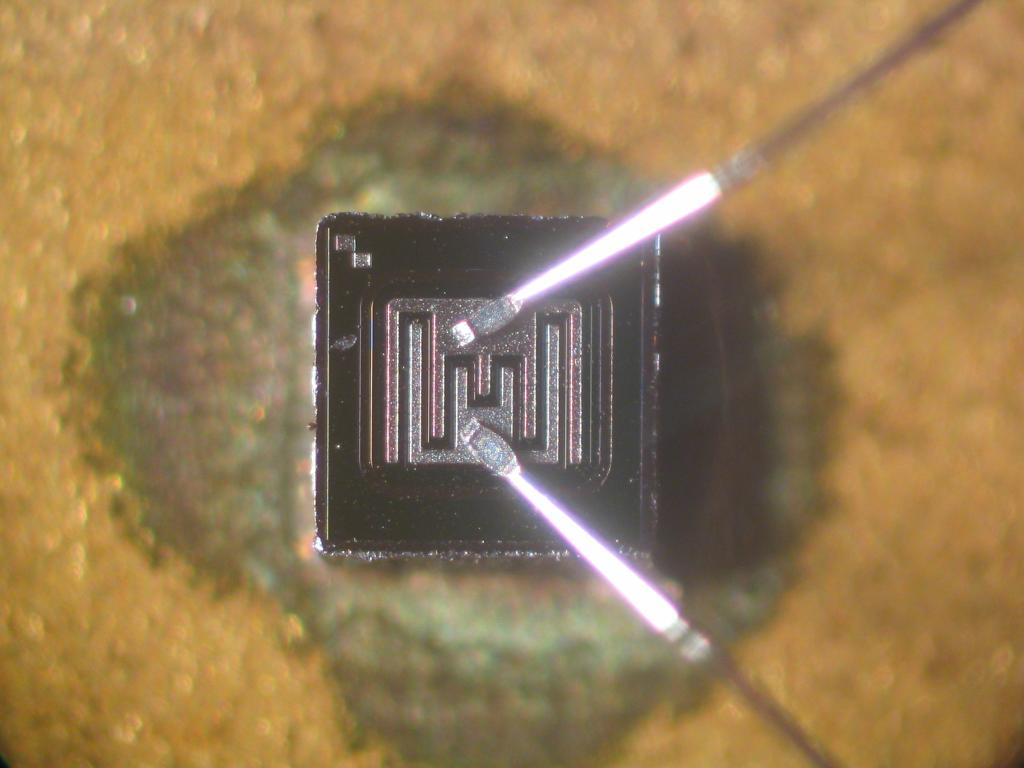
\includegraphics[scale=0.33]{pic/transistor}
\end{center}
}


\slide{Keeping space for images}
{
\begin{block}{Note}
Thanks to usage of \texttt{onslide} image sizes are preserved, even if not displayed.
Reserving space means things do not float between slide changes.
\end{block}

\begin{columns}

\begin{column}{0.33\textwidth}
\begin{center}
Column 1
\end{center}
\end{column}

\begin{column}{0.33\textwidth}
\begin{center}
Column 2
\end{center}
\end{column}

\begin{column}{0.33\textwidth}
\begin{center}
Column 3
\end{center}
\end{column}

\end{columns}

\begin{columns}

\begin{column}{0.33\textwidth}
\begin{center}
\onslide<2->{ \insImgCenter{0.1}{pic/transistor} }
\end{center}
\end{column}

\begin{column}{0.33\textwidth}
\begin{center}
\onslide<3->{ \insImgCenter{0.2}{svg/biohazard} }
\end{center}
\end{column}

\begin{column}{0.33\textwidth}
\begin{center}
\onslide<4->{ \insImgCenter{0.6}{pic/plantuml_logo} }
\end{center}
\end{column}

\end{columns}
}

\section{PlantUML}


\slide{UML diagrams}
{
\begin{center}

\includegraphics[scale=0.25]{pic/plantuml_logo}
\end{center}
\begin{itemize}
\item Generates UMLs
\item Input are text files
\item '\textbf{plantuml}' packages is needed
\item \texttt{apt-get install plantuml}
\item Syntax -- \url{http://plantuml.com/}
\end{itemize}
}


\slide{Activity diagram}
{
\begin{center}
\includegraphics[scale=0.25]{plantuml/activity_diagram}
\end{center}
}


\slide{Class diagram}
{
\begin{center}
\includegraphics[scale=0.25]{plantuml/class_diagram}
\end{center}
}


\slide{Object diagram}
{
\begin{center}
\includegraphics[scale=0.25]{plantuml/object_diagram}
\end{center}
}


\slide{Sequence diagram 1}
{
\begin{center}
\includegraphics[scale=0.25]{plantuml/sequence_diagram_1}
\end{center}
}


\slide{Sequence diagram 2}
{
\begin{center}
\includegraphics[scale=0.25]{plantuml/sequence_diagram_2}
\end{center}
}


\slide{State diagram}
{
\begin{center}
\includegraphics[scale=0.25]{plantuml/state_diagram}
\end{center}
}


\slide{Usecase diagram}
{
\begin{center}
\includegraphics[scale=0.25]{plantuml/usecase_diagram}
\end{center}
}

\section{Graphviz}


\slide{Hello world}
{
\vspace{-1em}
\begin{center}
% NOTE: explain diagram in depth
\includegraphics[scale=0.8]{dot/sample}
\end{center}
}


\slide{Diagrams with seqdiag}
{
\vspace{-1em}
\begin{center}
\includegraphics[scale=0.5]{dot/connection}
\end{center}
}

\section{Dia}


\slide{Dia image}
{
\begin{center}
\includegraphics[scale=0.6]{dia/example}
\end{center}
}

\section{Gnuplot}


\slide{Function plot}
{
\begin{center}
\includegraphics[scale=0.7]{gnuplot/function}
\end{center}
}


\slide{Discrete plot}
{
\begin{center}
\includegraphics[scale=0.55]{gnuplot/points}
\end{center}
}

\section{Generating codes}


\slide{QR}
{
\begin{itemize}
\item QR codes are auto-generated
\item Put \emph{txt} file in \emph{qr/} directory
\item Insert text there
\item Image will be auto-generated
\end{itemize}

\begin{center}
% NOTE: explain diagram in depth
\includegraphics[scale=0.1]{qr/some_info}
\end{center}
}

